% This is a LaTeX thesis template for Monash University.
% to be used with Rmarkdown
% This template was produced by Rob Hyndman
% Version: 6 September 2016

\documentclass{monashthesis}

%%%%%%%%%%%%%%%%%%%%%%%%%%%%%%%%%%%%%%%%%%%%%%%%%%%%%%%%%%%%%%%
% Add any LaTeX packages and other preamble here if required
%%%%%%%%%%%%%%%%%%%%%%%%%%%%%%%%%%%%%%%%%%%%%%%%%%%%%%%%%%%%%%%

\author{Dewi Lestari Amaliah}
\title{Thesis title}
\studentid{31251587}
\def\degreetitle{Master of Business Analytics}
% Add subject and keywords below
\hypersetup{
     %pdfsubject={The Subject},
     %pdfkeywords={Some Keywords},
     pdfauthor={Dewi Lestari Amaliah},
     pdftitle={Thesis title},
     pdfproducer={Bookdown with LaTeX}
}


\bibliography{thesisrefs}

\begin{document}

\pagenumbering{roman}

\titlepage

{\setstretch{1.2}\sf\tighttoc\doublespacing}

\clearpage\pagenumbering{arabic}\setcounter{page}{0}

\hypertarget{abstract}{%
\chapter*{Abstract}\label{abstract}}
\addcontentsline{toc}{chapter}{Abstract}

The abstract should outline the main approach and findings of the thesis and must not be more than 500 words.

\newpage

\hypertarget{acknowledgements}{%
\chapter*{Acknowledgements}\label{acknowledgements}}
\addcontentsline{toc}{chapter}{Acknowledgements}

I would like to thank my pet goldfish for \dots

\hypertarget{ch:intro}{%
\chapter{Introduction}\label{ch:intro}}

Start with visualisation
And then survey
And MRP

\hypertarget{sec:syslitrev}{%
\chapter{Systematic Literature Review}\label{sec:syslitrev}}

This study is performed using a systematic review method in which an attempt is made to collect empirical evidence explicitly and systematically using pre-specified eligibility criteria to answer a specific research question \autocite{cochrane}. Systematic literature review also enable the process of finding the gap in certain field of science, in terms of what has been done and what needs to be done \autocite{LinnenlueckeMartinaK2020Cslr}. Hence, in this case, systematic literature review could assist us to understand the common practice in MRP visualisations and how can we improve that.

According to \textcite{brown_uni}, the key criteria of the systematic literature review are: \emph{``a clearly defined question with inclusion \& exclusion criteria; rigorous \& systematic search of the literature; critical appraisal of included studies; data extraction and management; analysis \& interpretation of results; and report for publication.''} Hence, to conform with these criteria, this study incorporates the Preferred Reporting Items for Systematic Reviews and Meta-Analysis (PRISMA)'s checklist and flow diagram. The following subsections discuss the steps conducted following those criteria.

\hypertarget{literature-identification}{%
\section{Literature Identification}\label{literature-identification}}

MRP is applied in various scientific fields, ranging from social and political science to public health. Therefore, to identify the literature, this study refers to research databases instead of field-specific journals. Those databases are JSTOR, EBSCO, and PubMed. The first two databases are chosen due to their broad range of field coverage, while the latter is chosen since MRP is sometimes also applied in the health and medical field. Choosing these databases also considers that heterogeneity of included studies is one of the important factors in a systematic literature review \autocite{SchweizerMarinL2017Apgt}.

Further, we identify the literature using the combination of several search terms. Mostly the search term includes the term ``multilevel regression'', ``post-stratification'', ``poststratification'', and ``multilevel model''. Our target literature is articles that are written in English. Regarding the time of publication, we exclude all of the publications before 1997 since the MRP method has not been developed in this period. Initially we included only the title/abstract when searching these databases. However, using this method limits the set of potential articles to only include those with the search term in the abstract/title. To rectify this, we also include a search with ``all field'' in the search criteria. Note that for EBSCO, we directly apply the search for all fields. The detailed literature identification is shown in Table \ref{tab:search-term}.

The total number of articles from this search criteria are 327. Next, we utilize the literature manager, EndNote X9, to manage these articles and to find duplicate articles. After removing those duplicate articles, we have 212 articles to be screened in the next stage.

\begin{landscape}\begin{table}

\caption{\label{tab:search-term}Detail of literature identification}
\centering
\resizebox{\linewidth}{!}{
\begin{tabular}[t]{l>{\raggedright\arraybackslash}p{15em}lllr}
\toprule
Database & Search Terms & Search Field & Inclusion & Exclusion & Number Returned\\
\midrule
JSTOR & (multilevel regression and poststratification) OR (“post-stratification”) & Abstract & Article, content I can access, English & anything before 1997 & 44\\
JSTOR & (("multilevel regression" AND ("post-stratification" OR Poststratification)) OR ("multilevel model" AND ("post-stratification" OR Poststratification))) & All field & Article, English & anything before 1997 & 142\\
EBSCO & "multilevel regression with post-stratification" OR "multilevel regression with poststratification" OR "multilevel regression and Poststratification" OR "multilevel regression and Post-stratification" & All field & Academic (Peer-Reviewed) Journals, English & anything before 1997 & 42\\
EBSCO & (multilevel regression AND post-stratification) OR (multilevel model AND post-stratification) OR (multilevel regression AND poststratification ) OR (multilevel model AND poststratification) & All field & Academic (Peer-Reviewed) Journals, English & anything before 1997 & 45\\
PubMed & "multilevel regression with post-stratification" OR "multilevel regression with poststratification" OR "multilevel regression and Poststratification" OR "multilevel regression and Post-stratification" & Title/Abstract & Article, English & anything before 1997 & 26\\
\addlinespace
PubMed & (multilevel regression AND post-stratification) OR (multilevel model AND post-stratification) OR (multilevel regression AND poststratification) OR (multilevel model AND poststratification) & All field & Article, English & anything before 1997 & 28\\
\bottomrule
\end{tabular}}
\end{table}
\end{landscape}

\hypertarget{screening-and-eligibility-criteria}{%
\section{Screening and Eligibility Criteria}\label{screening-and-eligibility-criteria}}

We screen all of the articles whether they fit the criteria to be included in the study or not. We find that 3 articles are apparently not research papers. Hence, there are 209 abstracts to be screened. To screen efficiently, we use two stages as follow.

\hypertarget{stage-1-review-of-abstracts}{%
\subsection{Stage 1: Review of abstracts}\label{stage-1-review-of-abstracts}}

In the first stage DA and LK independently review all articles abstracts with the following eligibility criteria:

\begin{enumerate}
\def\labelenumi{\arabic{enumi}.}
\tightlist
\item
  The abstract should mentions analysis of data or creation of simulation data.
\item
  The abstract should mentions use of MRP or multilevel models to make population estimates or the use of other regression models (BART, spatial, stacked, trees) to make population estimates.
\end{enumerate}

During the screening, we agreed that 61 articles meet the eligibility criteria listed above, while 104 articles do not meet the criteria. Further, we disagreed on 44 articles. Accordingly, DA and LK skim the full manuscript to decide whether the paper could be included in the next stage or not. As the result, we include 22 more articles to be reviewed in stage 2.

\hypertarget{stage-2-full-manuscript-review}{%
\subsection{Stage 2: Full manuscript review}\label{stage-2-full-manuscript-review}}

DA reviews the full manuscript on 83 articles meet a second, more specific criteria. The aim of this stage is to get the list of the final articles that would be included in the study. We set the criteria of inclusion as follow:

\begin{enumerate}
\def\labelenumi{\arabic{enumi}.}
\tightlist
\item
  It should apply MRP as its method.
\item
  It should contain at least one plot relate to MRP findings.
\end{enumerate}

During this stage, we exclude 4 articles as they do not meet the first criteria. Further, 7 articles are excluded as they do not meet the second criteria. Also, an article is not included because it is a duplicate from other article that is already in the eligible list. However, this duplicate was not detected automatically by Endnote X9. Finally, we have 71 articles to be reviewed in the next stage. Figure \ref{fig:prisma-flowchart} displays the PRISMA flow chart of this study. This figure is generated using \texttt{PRISMA2020} \autocite{prisma2020}.

\begin{figure}
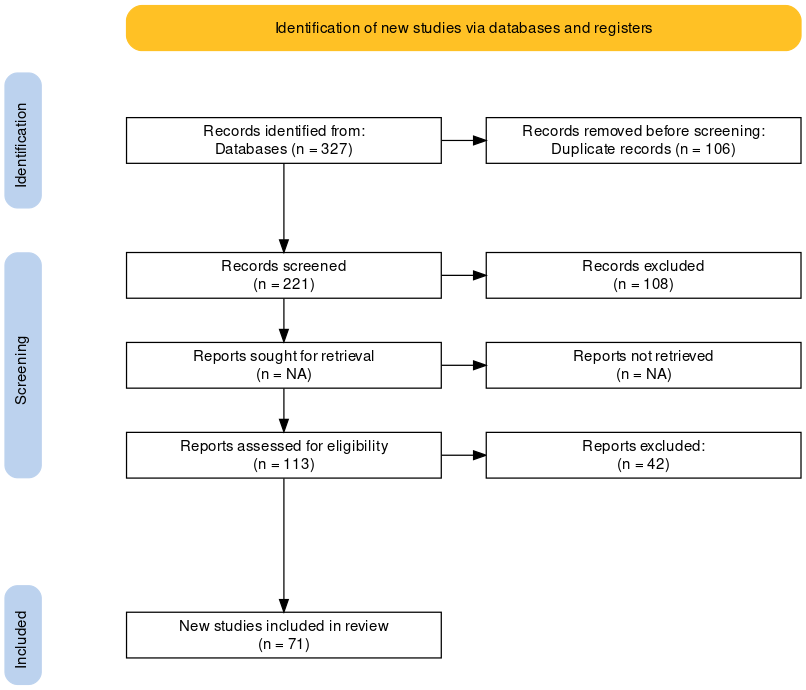
\includegraphics[width=0.9\linewidth]{figures/prisma_fc} \caption{PRISMA flow chart of this systematic literature review.}\label{fig:prisma-flowchart}
\end{figure}

\hypertarget{data-extraction-and-analysis}{%
\section{Data Extraction and Analysis}\label{data-extraction-and-analysis}}

We focus the data extraction on the MRP-related plot. We manually create a metadata for each plot (included in the supplementary material). We will use this metadata to analyse the current reporting practices with MRP. Besides, this metadata ensures the reproducibility of the analysis and to maintain the transparency of the systematic literature review process.

We code the plots according to their type, i.e., communication (coded to 0) and diagnostic plot (coded to 1). For diagnostic plots, we examine whether the plots compare MRP with other estimates, which are:

\begin{enumerate}
\def\labelenumi{\arabic{enumi}.}
\tightlist
\item
  Raw (direct estimates or direct disaggregation);
\item
  Ground truth;
\item
  Weight estimation;
\item
  Estimates of other MRP models, for example, the paper build several MRP models from various simulation scenarios or using different covariates;
\item
  Estimates from another study/survey;
\item
  Estimates from another method, for example comparing MRP with Bayesian Additive Tress with Post-Stratification.
\end{enumerate}

Plots that show a comparison of MRP with the above list would be coded to 1, otherwise coded to 0.
The diagnostic plot could also display the performance of MRP using these performance criteria:

\begin{enumerate}
\def\labelenumi{\arabic{enumi}.}
\tightlist
\item
  Bias;
\item
  Mean Absolute Error (MAE);
\item
  Mean Square Error (MSE)/ Relative Mean Square Error (RMSE);
\item
  Standard Error (SE);
\item
  Correlation.
\end{enumerate}

Just like the comparison, the MRP-related plot would be reviewed whether it is contains each of those metrics (coded 1) or not (coded 0).

We also review other features of the plot using the grammar in \texttt{ggplot2} \autocite{ggplot2}. The common grammar used in practice allows us to understand to what extend MRP models are effectively visualised. It is worth noting that there is no specific convention or well-documented recommendation on how data should be visualised as building a graph more often involve choice or preference \autocite{MIDWAY2020100141}. For example, there is no specific convention on which variable should be put on the x and y-axis in a scatter plot, even though it has been common knowledge to put the response variable on the y-axis and the explanatory variable on the x-axis. Hence, grammar assists us in evaluating well-formed graphics \autocite{layered-grammar}. In addition, \textcite{vanderplas} mention that classifying and comparing graphs according to their grammar is more robust and more elegant.

Accordingly, we examine the facet, geom, axis, color, and shape. Besides, the metadata also contains the article's author/s, article's year, article's title, and figure's number as appearing in the article. After the extraction, we analyze the data using graphical visualization with \texttt{ggplot2}. The result will be discussed in the following subsection.

\hypertarget{common-practices-in-mrp-visualisations}{%
\section{Common practices in MRP visualisations}\label{common-practices-in-mrp-visualisations}}

From 71 articles, we extract the data of 243 plots. 46.91 \% of these plots are diagnostics plots, while the remaining are communication plots.

\hypertarget{performance-metrics-used-in-mrp}{%
\subsection{Performance metrics used in MRP}\label{performance-metrics-used-in-mrp}}

\begin{figure}
\centering
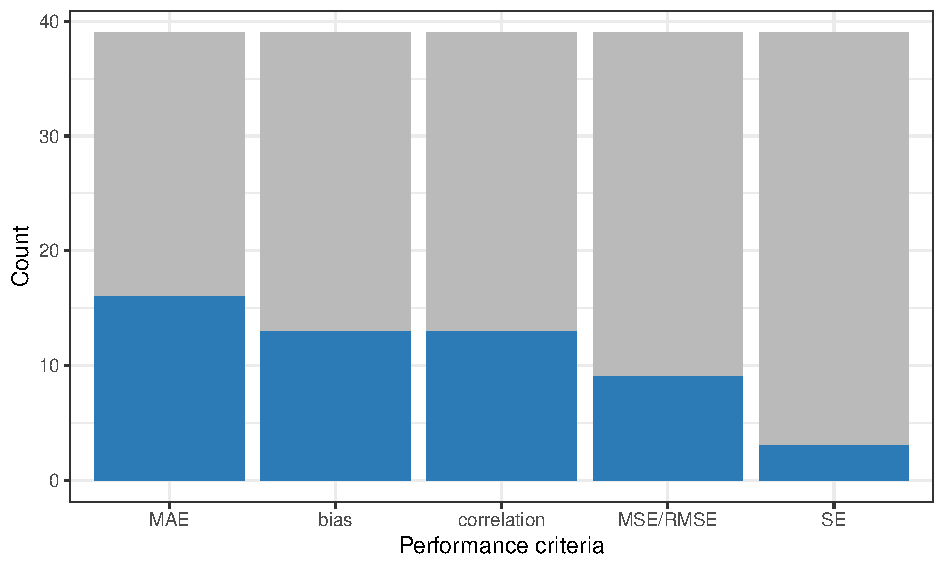
\includegraphics{thesis_files/figure-latex/perform-plot-1.pdf}
\caption{\label{fig:perform-plot}Metrics used as MRP performance criteria.}
\end{figure}

\hypertarget{common-estimates-to-compare-with-mrp-estimates}{%
\subsection{Common estimates to compare with MRP estimates}\label{common-estimates-to-compare-with-mrp-estimates}}

\begin{figure}
\centering
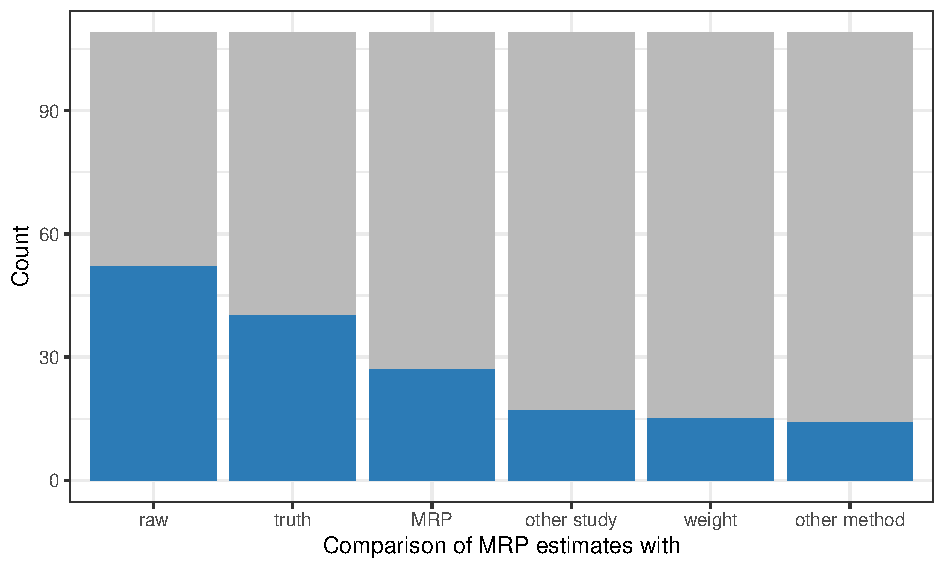
\includegraphics{thesis_files/figure-latex/compare-plot-1.pdf}
\caption{\label{fig:compare-plot}Estimates to compare with MRP.}
\end{figure}

\hypertarget{common-grammar-in-mrp-visualisations}{%
\subsection{Common grammar in MRP visualisations}\label{common-grammar-in-mrp-visualisations}}

\textbf{Plot type}

Plot type, referred as \texttt{geom} in grammar of graphics represents

\begin{figure}
\centering
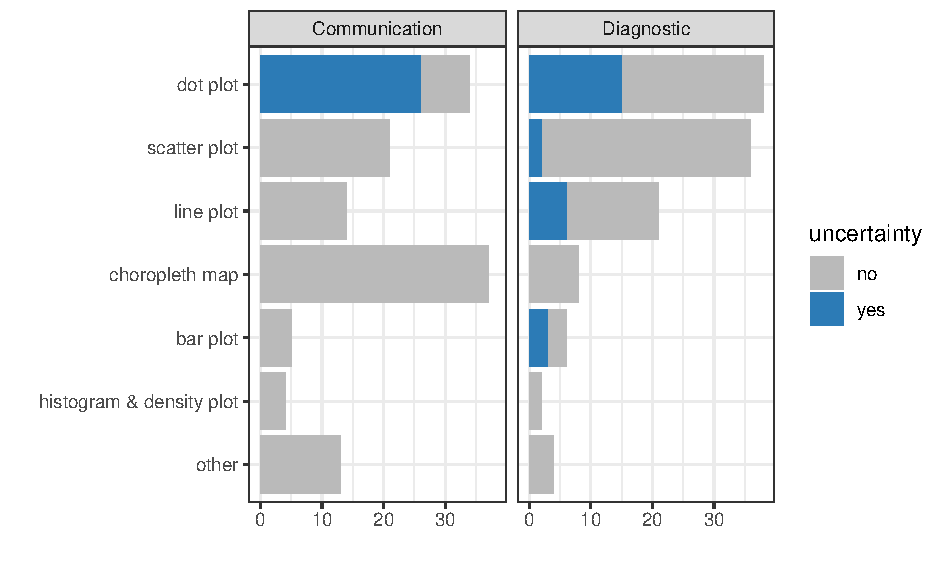
\includegraphics{thesis_files/figure-latex/common-plots-1.pdf}
\caption{\label{fig:common-plots}Common plot types used in MRP visualisations. Both communication and diagnostics plots rarely displayed uncertainty.}
\end{figure}

\textbf{Values put in x and y-axis}

\begin{figure}
\centering
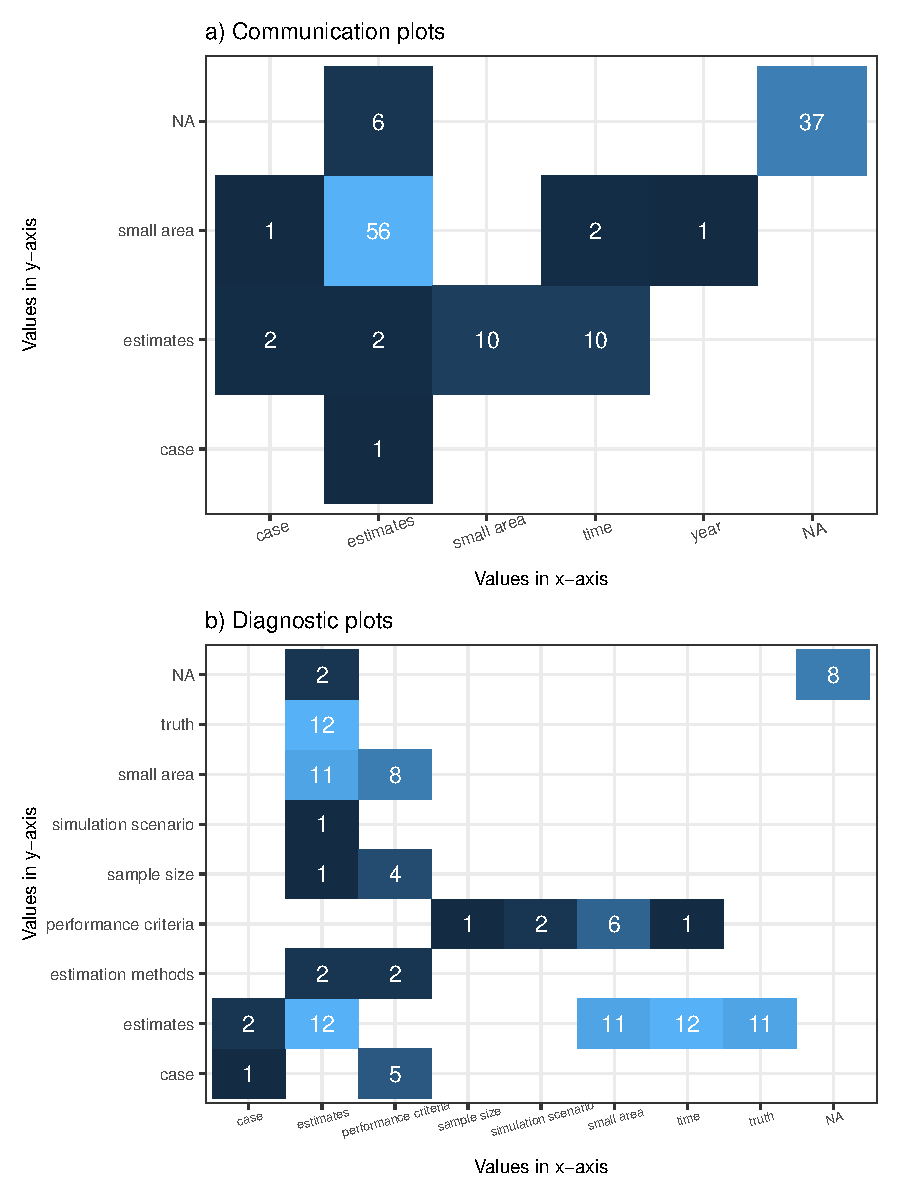
\includegraphics{thesis_files/figure-latex/common-axis-1.pdf}
\caption{\label{fig:common-axis}Common values put in plots' axis. Axis in diagnostic plots more varied compared to communication plot.}
\end{figure}

\textbf{Feature used}

\appendix

\hypertarget{additional-stuff}{%
\chapter{Additional stuff}\label{additional-stuff}}

You might put some computer output here, or maybe additional tables.

Note that line 5 must appear before your first appendix. But other appendices can just start like any other chapter.

\printbibliography[heading=bibintoc]



\end{document}
